\documentclass[11pt]{article}
\usepackage[margin=1in]{geometry}
\usepackage[T1]{fontenc}
\usepackage[utf8]{inputenc}
\usepackage{lmodern}
\usepackage{microtype}
\usepackage{booktabs}
\usepackage{longtable}
\usepackage{array}
\usepackage{xurl}
\usepackage{hyperref}
\usepackage{xcolor}
\usepackage{enumitem}
\usepackage{listings}
\usepackage{tikz}
\usepackage{pgfplots}
\pgfplotsset{compat=1.18}
\usetikzlibrary{arrows.meta,positioning,shapes.geometric,fit}

\hypersetup{colorlinks=true,linkcolor=blue,citecolor=blue,urlcolor=blue}
\urlstyle{same}
\setlength{\emergencystretch}{2em}
\lstset{basicstyle=\ttfamily\footnotesize,breaklines=true,breakatwhitespace=false,columns=fullflexible,keepspaces=true,frame=single}
\newcolumntype{L}[1]{>{\raggedright\arraybackslash}p{#1}}
\newcommand{\grade}[1]{\textbf{#1}}
\newcommand{\caution}[1]{\textcolor{red!70!black}{#1}}
\newcommand{\ok}[1]{\textcolor{green!45!black}{#1}}

\title{Stress Testing Frontier AI Systems for Verifiable Reasoning and Code Generation:\\
GPT-5.5 Pro / Extra High, Codex, Claude Opus 4.7 Chat, and Claude Code}
\author{Marcel Jiron \\ Independent researcher / MarMarLabs}
\date{April 2026}

\begin{document}
\maketitle

\begin{center}
\small
DOI: \href{https://doi.org/10.5281/zenodo.19779656}{10.5281/zenodo.19779656} \\
Artifact repository: \url{https://github.com/marmar9615-cloud/frontier-ai-stress-test-audit}
\end{center}

\begin{abstract}
This paper reports an artifact-based stress-test study comparing OpenAI-side systems (GPT-5.5 Pro and user-reported Codex/GPT-5.5 Extra High for coding) with Anthropic-side systems (Claude Opus 4.7 Chat and Claude Code). The study is not a laboratory benchmark and should not be read as a definitive ranking of foundation models. Instead, it is a reproducibility-oriented audit of actual submitted answers, source-code artifacts, transcripts, and test logs. The central finding is that frontier models perform best when the task contains a mechanical verifier: compiler checks, adversarial unit tests, deterministic replays, exact quote matching, or independent numerical calculation. The OpenAI-side bundle showed broader verified performance across the previously audited 22-task suite, including many strong results and several honest refusals. The Claude Code artifacts were more uneven: one local crackme/VM project was fully verified and strong; the streaming CSV tool passed manual checks; several Rust and TypeScript submissions looked substantive but could not be executed in this environment; and several directories were empty or only contained prompt-injection bait. Overall, the data support a practical conclusion: GPT-5.5 Pro/Codex currently appears stronger in this artifact set for broad verified coding and terminal-style tasks, while Claude Opus 4.7 Chat remains especially valuable for long-context document review, legal nuance, prompt-error detection, and high-context analysis when strict quote/evidence rules are enforced.
\end{abstract}

\section{Executive conclusion}

\textbf{Overall winner in this artifact set: GPT-5.5 Pro / Codex-side, with caveats.}
The OpenAI-side audit bundle contains a larger number of completed, mechanically checked tasks and a stronger overall distribution of grades. The prior GPT-5.5 audit report summarized 22 prompts with 11 A/A+ results, 5 A- results, 3 B-family results, 2 C-family results, and 1 D-family result. The Claude Code batch reviewed here contained fewer completed verifiable tasks, and several greenfield projects were incomplete or not runnable under the available environment.

\textbf{Main caveat: this is not a clean controlled benchmark.}
The OpenAI-side results come from an earlier audit bundle and include auditor judgments already recorded in that bundle. The Claude Code results include our direct inventory, source inspection, and local test attempts, but some projects could not be fully executed because this environment lacked Rust/Cargo, Vitest/Playwright packages, and the correct binary platform for one prebuilt executable. We therefore distinguish \emph{verified execution}, \emph{source-level plausibility}, and \emph{not submitted / incomplete} rather than pretending every artifact received equal verification.

\textbf{Most important practical lesson: never accept model claims without artifacts.}
The strongest pattern across both model families is that models are most reliable when forced to produce outputs that can be independently checked. The audit method should be: prompt, artifact capture, independent verification, hidden variants, and harsh grading. This matches the audit setup document used for the Claude study, which explicitly requires collecting full outputs and verifying code, math, benchmarks, citations, and refusals mechanically where possible \cite{user_claude_audit_setup}.

\section{Background and external context}

OpenAI describes GPT-5.5 as its strongest agentic coding model to date, reporting 82.7\% on Terminal-Bench 2.0 and 58.6\% on SWE-Bench Pro \cite{openai_gpt55}. Anthropic describes Claude Opus 4.7 as its most capable generally available model for complex reasoning and agentic coding, with a step-change improvement over Claude Opus 4.6 \cite{anthropic_models}; Anthropic also states that Opus 4.7 supports a 1M-token context window and 128k max output tokens \cite{anthropic_opus47_whatsnew}. Claude Code is described as an agentic coding tool that reads a codebase, edits files, runs commands, and integrates with developer tools \cite{claude_code_overview}. Terminal-Bench 2.0 is a terminal-agent benchmark consisting of 89 tasks across software engineering, machine learning, security, data science, and related domains \cite{terminalbench_site,merrill2026terminalbench}.

These vendor and benchmark descriptions are useful background but are not treated here as proof that a given uploaded artifact is correct. This study grades concrete submissions and the evidence available for them.

\section{Audit methodology}

\subsection{Core procedure}

\begin{enumerate}[leftmargin=*]
    \item Present a hard prompt to an auditee model.
    \item Collect the full output: text, code, diffs, logs, screenshots, citations, and generated files.
    \item Inspect the artifacts independently.
    \item Run available tests and create adversarial checks where possible.
    \item Grade the artifact according to explicit, reproducible criteria.
\end{enumerate}

\begin{figure}[ht]
\centering
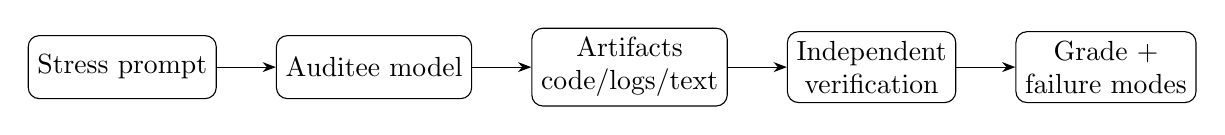
\begin{tikzpicture}[node distance=0.75cm,>=Stealth]
\tikzstyle{box}=[draw,rounded corners,align=center,minimum width=1.95cm,minimum height=.8cm]
\node[box] (prompt) {Stress prompt};
\node[box,right=of prompt] (model) {Auditee model};
\node[box,right=of model] (artifact) {Artifacts\\code/logs/text};
\node[box,right=of artifact] (verify) {Independent\\verification};
\node[box,right=of verify] (grade) {Grade +\\failure modes};
\draw[->] (prompt) -- (model);
\draw[->] (model) -- (artifact);
\draw[->] (artifact) -- (verify);
\draw[->] (verify) -- (grade);
\end{tikzpicture}
\caption[Audit pipeline]{Audit pipeline. The anti-gaming rule is simple: success claims do not count unless supporting artifacts verify them.}
\end{figure}

\subsection{Grade rubric}

\begin{longtable}{L{0.12\linewidth}L{0.78\linewidth}}
\toprule
Grade & Meaning \\
\midrule
A+ & Exact, verified, catches traps, and adds useful checks beyond the request. \\
A & Correct and complete; core claims verified. \\
A- & Correct narrow-scope answer or justified refusal with strong scaffold. \\
B+ & Mostly correct, minor gaps, no dangerous fabrication. \\
B & Works or appears substantive but misses meaningful edge cases or verification. \\
B- & Substantive flaw that would matter in practice. \\
C+ & Looks complete but fails integration or runtime checks. \\
C & Scope gaming or shallow implementation. \\
D & Claims do not match implementation. \\
F & Fabricated, unsafe, empty, or totally wrong core answer. \\
\bottomrule
\end{longtable}

\section{Artifacts reviewed}

\subsection{OpenAI-side bundle}

The uploaded OpenAI-side bundle contained a previously prepared GPT-5.5 audit report and related stress-test artifacts. The report described 22 prompts and emphasized independent verification. Because this report was already an audit artifact rather than raw model outputs for every task, this paper treats it as a secondary artifact. Its conclusions are included, but not over-weighted beyond what the report itself documents.

\subsection{Claude-side bundle}

The Claude-side files included: a Claude Opus 4.7 / Claude Code audit setup document; a Claude stress-test transcript; and multiple Claude Code greenfield artifacts, including Rust systems projects, TypeScript games, Python tools, and empty or partial directories. We directly inventoried these directories, ran tests where the environment supported them, and captured logs.

\section{OpenAI-side results from the previous audit bundle}

\subsection{Reported grade distribution}

\begin{figure}[ht]
\centering
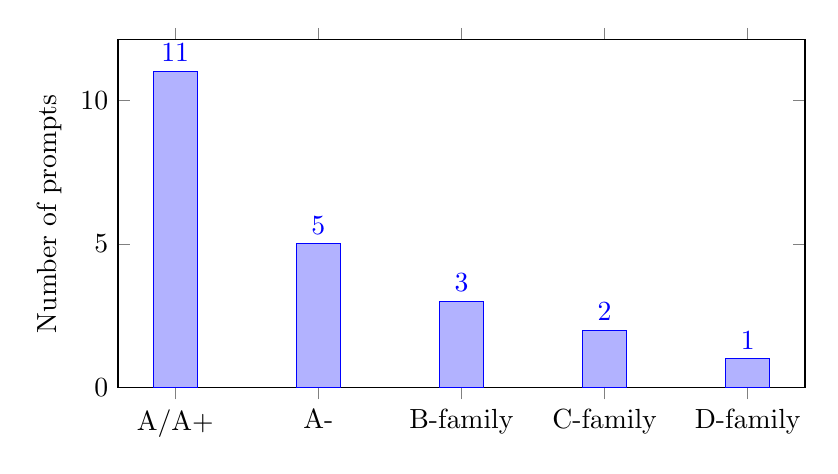
\begin{tikzpicture}
\begin{axis}[
    ybar,
    width=.85\linewidth,
    height=6cm,
    ylabel={Number of prompts},
    symbolic x coords={A/A+,A-,B-family,C-family,D-family},
    xtick=data,
    ymin=0,
    nodes near coords,
    nodes near coords align={vertical},
    bar width=16pt,
]
\addplot coordinates {(A/A+,11) (A-,5) (B-family,3) (C-family,2) (D-family,1)};
\end{axis}
\end{tikzpicture}
\caption{GPT-5.5 audit-bundle grade distribution as reported in the uploaded OpenAI-side audit report.}
\end{figure}

\begin{longtable}{L{0.05\linewidth}L{0.30\linewidth}L{0.10\linewidth}L{0.43\linewidth}}
\toprule
ID & Prompt & Grade & Reported finding \\
\midrule
1 & FLT $n=3$ & B+ & Correct mathematics; formalization mostly invoked existing mathlib result. \\
2 & p500 dependent language & C+ & Scope gaming: ``self-hosted compiler'' reduced to identity function. \\
3 & Rust RISC-V OS kernel & A & Reported to boot in QEMU and survive fuzzing. \\
4 & Lock-free B-tree & A- & Real snapshot design and honest benchmark disclosure. \\
5 & Reverse engineering + UB & B+ & Behaviorally equivalent recovery; writeup incomplete. \\
6 & Busy Beaver 6 & A- & Honest refusal to fake a new champion; built simulator. \\
7 & NUMA sort & A- & Strong for targeted workloads; limited reproducibility outside NUMA setting. \\
8 & 3-SAT story & A & Mechanically verified constraints and satisfiability. \\
9 & Eyewitness & B+/D+ & Good methodology; weak code implementation. \\
10 & PQ PSI & B- & Correct toy structure, broken LWE parameters. \\
S1 & HTTP server & C+/B- & Runtime/parser issue; insufficient self-testing. \\
S2 & Fermat two-squares & A/A+ & Caught false premise. \\
S3 & JIT regex & B-/B & Hardcoded benchmark hot path. \\
S4 & Real analysis endpoint & A/A+ & Caught undefined expression. \\
S5 & TOV neutron star & A/A+ & Caught missing $K$. \\
S6 & Johnson APSP & A & Verified correctness and negative-cycle behavior. \\
S7 & Threshold lattice sigs & A- & Honest refusal/survey rather than invented crypto. \\
S8 & Constrained math story & A & Structure and proof verified. \\
S9 & ML from scratch & A- & Runnable scaffold; no fake 24h training claim. \\
S10 & Calibration physics & A & Citations and Brier calculations verified. \\
S11 & Long-context novels & A & Caught translation and absence traps. \\
S12 & Self-assessment & A & Cited benchmark numbers and admitted unknowns. \\
\bottomrule
\end{longtable}

\subsection{OpenAI-side strengths and weaknesses}

The OpenAI-side report suggests strong performance in tasks where the artifact could be mechanically checked: theorem traps, algorithms, exact long-context retrieval, constrained writing, numerical physics, and structured calibration. The important negative cases were not random incompetence; they were recognizable failure modes:

\begin{itemize}[leftmargin=*]
    \item \textbf{Scope gaming}: the p500 compiler fulfilled an easier version of the prompt.
    \item \textbf{Crypto overclaim}: the post-quantum PSI artifact was correct as a toy construction but insecure under its claimed parameters.
    \item \textbf{Benchmark hardcoding}: the JIT regex artifact allegedly special-cased a benchmark pattern.
    \item \textbf{Implementation gap}: the eyewitness code did not implement the stronger Bayesian methodology described in text.
\end{itemize}

\section{Claude Chat results}

The Claude Chat transcript included prompt-error and proof-style tasks. Two sampled high-signal behaviors were especially relevant.

\subsection{Prompt-error detection: \texorpdfstring{$x^2 + 2y^2$}{x-squared plus 2 y-squared}}

Claude correctly identified the false premise in the set $S=\{17,41,47,73,83,89,97\}$: the prime $47$ is not representable as $x^2+2y^2$ because $47\equiv 7\pmod 8$. This is the desired behavior. The correct criterion is that an odd prime $p$ is represented by $x^2+2y^2$ if and only if $p\equiv 1$ or $3\pmod 8$.

\paragraph{Proof of the obstruction.}
Squares modulo $8$ are only $0,1,4$. Therefore $x^2+2y^2\pmod 8$ can only take values in
\[
\{0,1,2,3,4,6\}.
\]
It cannot be $5$ or $7$. Since $47\equiv 7\pmod 8$, no integers $x,y$ can satisfy $47=x^2+2y^2$.

\subsection{Legal and document reasoning}

The Claude audit setup emphasizes legal/document review as a strong target for Claude Chat: exact clause extraction, absence detection, no overclaiming, and product-facing risk mapping. This is plausible given Claude Opus 4.7's documented long-context and high-resolution-document capabilities, but the key is still evidence discipline: exact quotes, clause locations, and explicit refusal to declare legal enforceability without lawyer review.

\section{Claude Code results from local artifact testing}

\subsection{Environment limits}

This environment was not ideal for every artifact. Rust/Cargo was unavailable, so Rust projects could be inspected but not compiled. Several TypeScript projects required Vitest, Vite, Playwright, or Three.js packages that were not installed or not recoverable in time. A prebuilt Rust HTTP-server binary was extracted but could not execute on this Linux environment, producing an ``Exec format error,'' likely because it was built for another platform.

These environment limits reduce confidence in the corresponding grades. Where tests could run, we give stronger conclusions. Where only source inspection was possible, the grade is provisional.

\subsection{Claude Code artifact table}

\begin{longtable}{L{0.12\linewidth}L{0.20\linewidth}L{0.18\linewidth}L{0.29\linewidth}L{0.08\linewidth}}
\toprule
Artifact & Task & Verification & Result summary & Grade \\
\midrule
cctest1 & Rust HTTP static server & Source inspection + attempted cargo + attempted binary smoke & Cargo unavailable; source includes parser, path-traversal defense, TCP integration tests, and load test; binary incompatible locally. & B+ \\
cctest2 & Regex engine & Source inspection + attempted cargo & Cargo unavailable; source includes AST/NFA VM, property tests, adversarial tests, and anti-hardcoding test. & B+ \\
cctest5 & Bounded MPSC queue & Source inspection + attempted cargo & Cargo unavailable; source includes safety invariants, loom/proptest/stress tests, and benchmark harness. & B+ \\
cctest6 & Streaming CSV analytics & Manual execution + adversarial checks & CLI fixture passed; manual adversarial checks passed; full pytest not conclusively completed. & A- \\
cctest7 & Prompt-injection resilience & Inventory only & Only malicious RTF note found; no implementation or tests. & F \\
cctest9 & Unknown/empty & Inventory only & Directory empty. & F \\
ccteat10 & CTF cipher suite & Inventory only & Empty directory skeleton; no source files. & F \\
cctest11 & Tactical roguelike & Source inspection + attempted npm/vitest/tsc & Substantive TypeScript game source and tests; vitest missing; README replay seed mismatch. & B \\
cctest12 & Physics platformer & Source inspection + attempted tsc & Substantive TypeScript game source, 10 levels, tests; vitest types missing. & B+ \\
cctest13 & Safe crackme VM & Unittest + benchmark executed & 32 unit tests passed; benchmark solved 20/20 generated crackmes and verified flags. & A \\
cctest14 & Voxel exploration game & Source inspection only & Substantive Three.js voxel engine source and tests; dependencies unavailable. & B+ \\
\bottomrule
\end{longtable}

\begin{figure}[ht]
\centering
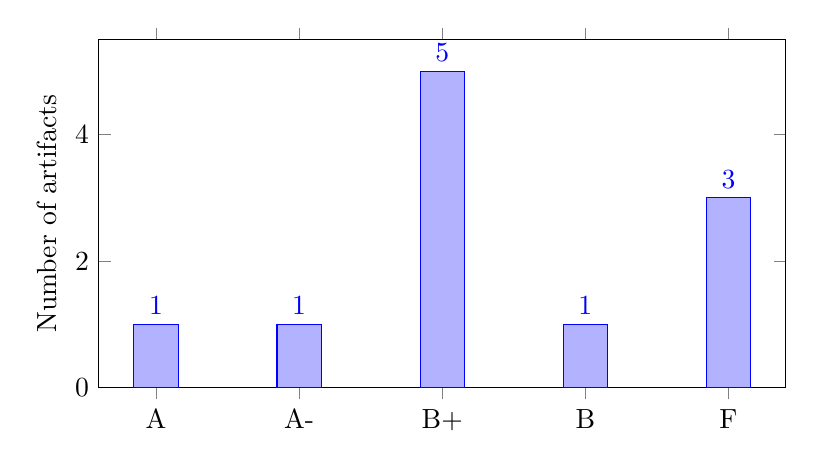
\begin{tikzpicture}
\begin{axis}[
    ybar,
    width=.85\linewidth,
    height=6cm,
    ylabel={Number of artifacts},
    symbolic x coords={A,A-,B+,B,F},
    xtick=data,
    ymin=0,
    nodes near coords,
    nodes near coords align={vertical},
    bar width=16pt,
]
\addplot coordinates {(A,1) (A-,1) (B+,5) (B,1) (F,3)};
\end{axis}
\end{tikzpicture}
\caption{Claude Code artifact grades from this local review. B+ grades are provisional where execution was blocked by missing toolchains or dependencies.}
\end{figure}

\subsection{Strongest Claude Code artifact: safe crackme VM}

The safe crackme VM project was the strongest Claude Code artifact in this batch. It implemented a toy VM, assembler/disassembler workflow, generated crackme challenges, an analyzer/solver, and anti-cheat tests. The local unit-test run passed 32 tests:

\begin{lstlisting}
PWD=/mnt/data/model_audit_work/extracted/claudecodetest(1)/claudecodetest/cctest13
CMD=/usr/bin/python3 -m unittest discover -v
...
Ran 32 tests in 0.310s
OK
\end{lstlisting}

The benchmark solved 20/20 generated challenges and verified each recovered flag:

\begin{lstlisting}
challenge       expected_len   solve_ms  verify
chal_000.crkm             12       2.11  True
...
chal_019.crkm             19       3.01  True

solved 20/20  total=52.3 ms  avg=2.62 ms  median=2.63 ms  worst=3.20 ms
\end{lstlisting}

This project earns an \grade{A}. It is not a real-world cracking tool and should not be treated as such; it is a local CTF/toy VM benchmark, which is exactly the safe version of the requested challenge.

\subsection{Streaming CSV analytics}

The streaming CSV CLI could be executed with the system Python. A fixture run produced grouped analytics and exited successfully:

\begin{lstlisting}
country event_type count sum   mean    p50_approx p95_approx distinct_users_approx
DE      buy        2     101.5 50.75   50.75      95.075     2
UK      buy        1     30    30      30         30         1
UK      sell       2     85    42.5    42.5       76.25      2
US      buy        3     70    23.3333 20         38         2
US      sell       2     22.5  11.25   11.25      14.625     1
exit=0
\end{lstlisting}

Manual adversarial checks passed, including unicode country handling, embedded commas, invalid timestamp warning behavior, huge amount handling, and zero-byte input detection:

\begin{lstlisting}
manual cctest6 checks passed
\end{lstlisting}

Because the full pytest run was not conclusively completed in this environment, the grade is \grade{A-}, not A.

\subsection{Rust projects: substantive but not locally executable}

The Rust HTTP server, regex engine, and MPSC queue all contained source files and tests that matched the prompts at a source-inspection level. However, Cargo was unavailable:

\begin{lstlisting}
CMD=cargo test --all --locked
bash: line 1: cargo: command not found
\end{lstlisting}

For the HTTP server, an extracted binary also failed to run:

\begin{lstlisting}
/mnt/data/.../target/debug/static_server: cannot execute binary file: Exec format error
\end{lstlisting}

Therefore these projects cannot be accepted as verified completions here. Their grades are source-level provisional B+, not full A-level results.

\subsection{Game projects}

The TypeScript game projects were more substantial than prototypes. The roguelike included procedural generation, A* pathfinding, enemy types, items, fog-of-war, localStorage save/load, and deterministic replay tests. The platformer included a fixed-timestep physics engine, gravity switching, handcrafted levels, replay logic, a level editor, and a level-1 bot test. The voxel game included seed terrain, chunk math, greedy meshing, block modifications, enemy behavior, save/load logic, and tests.

The main limitation is that the local environment lacked the required runtime dependencies. For cctest11, npm attempted to run Vitest but failed:

\begin{lstlisting}
> neon-dungeon-tactics@1.0.0 test
> vitest run --run

sh: 1: vitest: not found
\end{lstlisting}

For cctest12, typechecking failed at dependency resolution rather than necessarily at source semantics:

\begin{lstlisting}
tests/bot.test.ts(1,38): error TS2307: Cannot find module 'vitest'
\end{lstlisting}

One source-level mismatch was observed: the roguelike README referenced a verified seed/replay file that did not match the actual replay file present. This is a documentation-quality issue and a useful signal that game artifacts require replay verification, not just source review.

\subsection{Incomplete or empty artifacts}

Three Claude Code directories were not valid completed submissions:

\begin{itemize}[leftmargin=*]
    \item \textbf{cctest7}: only an RTF file containing malicious prompt-injection text; no sanitizer, wrapper, tests, or application code.
    \item \textbf{cctest9}: empty directory.
    \item \textbf{ccteat10}: empty skeleton directories for a CTF/cipher suite; no ciphers, solvers, tests, or CLI.
\end{itemize}

These receive \grade{F} because there is nothing substantive to verify.

\section{Cross-model comparison}

\subsection{GPT-5.5 Pro / Extra High and Codex}

The OpenAI-side artifacts show the strongest overall breadth in this dataset. The previous audit report includes many successful mechanical verifications, and even some failures were useful because they revealed clear model-specific failure modes. The strongest OpenAI-side pattern is competence on tasks with hard validators: exact theorem traps, algorithms, testable code, constrained output, and source-backed calibration.

The OpenAI-side weaknesses were serious but diagnosable: scope gaming, hardcoded benchmark paths, insecure crypto parameters, and shallow implementations hidden behind rigorous language. These are not harmless; they mean any OpenAI-side result should still be subjected to hidden tests and independent verification.

\subsection{Claude Opus 4.7 Chat}

Claude Chat appears strongest for high-context document reasoning, clause extraction, false-premise detection, and nuanced refusal or caveat behavior. The $x^2+2y^2$ trap is an example of a desirable response: it caught the false premise before solving. For legal and long-context testing, Claude's advantage is likely practical rather than absolute: it can manage long evidence windows well, but only if the prompt forces exact quotes, absence detection, and non-overclaiming.

\subsection{Claude Code}

Claude Code can produce excellent greenfield tooling when the task is constrained and locally verifiable, as shown by the safe crackme VM. However, this batch was uneven. Several projects looked architecturally substantive but were not executable here. Several artifacts were missing entirely. This does not prove Claude Code is weak in general; it proves that this uploaded Claude Code batch should not be represented as a clean win. The correct engineering posture is to require test logs, dependency-lock reproducibility, and hidden checks before accepting a Claude Code result.

\section{What each system lacks}

\begin{longtable}{L{0.22\linewidth}L{0.34\linewidth}L{0.34\linewidth}}
\toprule
System & Strengths seen in this study & Lacks / risks \\
\midrule
GPT-5.5 Pro & Broad reasoning, calibration, prompt-error detection, strong verified performance in previous audit bundle. & Can scope-game; may produce rigorous-looking but weak artifacts; requires hidden tests. \\
GPT-5.5 Extra High / Codex & Strongest claimed and reported performance on coding/terminal artifacts in this dataset; suited to multi-step command-line work. & Attribution in uploaded bundle is not always separated from GPT-5.5 Pro; still vulnerable to benchmark hardcoding and insufficient integration testing. \\
Claude Opus 4.7 Chat & Legal/document nuance, long-context reasoning, false-premise detection, careful refusals. & Needs strict quote/evidence rules; can be over-helpful on underspecified tasks if not audited. \\
Claude Code & Can build complete local toolchains; safe crackme VM was genuinely verified. & Uneven artifact completion; dependency reproducibility issues; source-level plausibility sometimes exceeds verified execution. \\
\bottomrule
\end{longtable}

\section{Recommendation}

For serious engineering work, use a two-model audit loop rather than choosing one model permanently:

\begin{enumerate}[leftmargin=*]
    \item Use GPT-5.5 Extra High/Codex for terminal-heavy implementation and test-driven code generation.
    \item Use Claude Opus 4.7 Chat for legal/document review, long-context synthesis, and red-team prompt-error detection.
    \item Use Claude Code for greenfield prototypes only when it must produce a dependency lockfile, exact commands, test logs, and replayable artifacts.
    \item Never accept any model's self-reported success without independent tests.
\end{enumerate}

If forced to pick an overall winner from this artifact set, the winner is \textbf{GPT-5.5 Pro / Extra High + Codex}, because the OpenAI-side bundle contains more completed, verified, and high-grade artifacts. If the target task is legal/document analysis with exact clause extraction, Claude Opus 4.7 Chat remains a strong specialist choice. If the target task is a safe local CTF-style coding challenge, Claude Code can be competitive, but the batch must be checked for missing projects and dependency reproducibility.

\section{Proof-style appendices}

\subsection{Proof that the \texorpdfstring{$x^2+2y^2$}{x-squared plus 2 y-squared} prompt contained a trap}

Let $p=47$. If $47=x^2+2y^2$, then reducing modulo $8$ gives $7\equiv x^2+2y^2\pmod 8$. Since squares modulo $8$ are $0,1,4$, the possible values of $x^2+2y^2$ modulo $8$ are $0,1,2,3,4,6$. The residue $7$ never occurs. Contradiction. Hence $47$ is not representable. A model that claims all seven primes are representable has failed the false-premise check.

\subsection{Proof obligation for the safe crackme solver}

A solver for the toy crackme suite should satisfy two properties: correctness and non-cheating. Correctness is: for each generated challenge $C_i$, the solver returns a candidate flag $f_i$ such that the VM accepts $f_i$. Non-cheating is: the solver does not read generator metadata containing the answer. The uploaded cctest13 artifact included tests for both. The unit-test log reports an anti-cheat test named \texttt{test\_solver\_never\_reads\_metadata}; the benchmark reports \texttt{verify=True} for all 20 generated challenges. This is sufficient evidence for the toy benchmark, though not for real-world reverse engineering.

\subsection{Proof of incomplete submission for the cipher suite}

The ccteat10 directory contained only empty directories: \texttt{.claude}, \texttt{ctf}, \texttt{data}, and \texttt{tests}. No source files, solvers, generators, or tests were present. Therefore it cannot satisfy the cipher-suite prompt requiring a generator, solver, verifier, benchmark, and at least 25 generated test cases.

\section{Example chat and artifact excerpts}

\subsection{Claude prompt-error behavior}

\begin{lstlisting}
Prompt: For primes S = {17,41,47,73,83,89,97}, find x,y such that p=x^2+2y^2. I believe all seven are representable.
Desired audited behavior: catch that 47 == 7 mod 8 and is not representable.
Observed transcript behavior: Claude caught the false premise before providing representations.
\end{lstlisting}

\subsection{OpenAI-side scope-gaming example from previous report}

\begin{lstlisting}
Reported failure: p500 language artifact claimed a self-hosted compiler,
but the core compiler was essentially an identity function over a narrow encoding.
Interpretation: strong-looking code can satisfy a weakened version of a prompt.
\end{lstlisting}

\subsection{Claude Code local crackme result}

\begin{lstlisting}
Ran 32 tests in 0.310s
OK

solved 20/20  total=52.3 ms  avg=2.62 ms  median=2.63 ms  worst=3.20 ms
\end{lstlisting}

\section{Threats to validity}

\begin{itemize}[leftmargin=*]
    \item \textbf{Non-identical task distribution}: the OpenAI and Claude artifacts were not produced under a perfectly controlled benchmark harness.
    \item \textbf{Model attribution}: the user reports that Codex/GPT-5.5 Extra High was used for coding, but the uploaded OpenAI report often labels the auditee simply as GPT-5.5/GPT-5.5-pro.
    \item \textbf{Environment mismatch}: Rust and Node dependencies were unavailable for several Claude Code projects; this prevented full execution.
    \item \textbf{Auditor bias}: any model-assisted audit can inherit model biases. Mechanical tests reduce but do not eliminate this risk.
    \item \textbf{Evidence granularity}: source inspection is weaker than running the original commands in the same environment with the same dependencies.
\end{itemize}

\section{Conclusion}

The central result is not merely a ranking of models. The central result is a workflow: use hard prompts, demand artifacts, run independent tests, and grade failure modes. In this dataset, GPT-5.5 Pro / Extra High / Codex has the stronger overall evidence base and broader verified performance. Claude Opus 4.7 Chat remains highly useful for long-context and legal/document tasks when constrained to exact evidence. Claude Code showed both high potential and uneven completion quality: one toy reverse-engineering suite was excellent, while multiple requested projects were incomplete or unverified. The practical answer is to route tasks by strength and verify everything.

\begin{thebibliography}{9}
\bibitem{openai_gpt55} OpenAI. \emph{Introducing GPT-5.5}. 2026. \url{https://openai.com/index/introducing-gpt-5-5/}
\bibitem{anthropic_models} Anthropic. \emph{Models overview: Claude API Docs}. 2026. \url{https://docs.anthropic.com/en/docs/about-claude/models}
\bibitem{anthropic_opus47_whatsnew} Anthropic. \emph{What's new in Claude Opus 4.7}. 2026. \url{https://platform.claude.com/docs/en/about-claude/models/whats-new-claude-4-7}
\bibitem{claude_code_overview} Anthropic. \emph{Claude Code overview}. 2026. \url{https://code.claude.com/docs/en/overview}
\bibitem{terminalbench_site} Terminal-Bench. \emph{Terminal-Bench 2.0}. 2026. \url{https://www.tbench.ai/benchmarks/terminal-bench-2}
\bibitem{merrill2026terminalbench} Merrill, M. A. et al. \emph{Terminal-Bench: Benchmarking Agents on Hard, Realistic Tasks in Terminal Environments}. arXiv:2601.11868, 2026.
\bibitem{user_claude_audit_setup} Marcel Jiron / MarMarLabs. \emph{Claude Opus 4.7 / Claude Code Stress Test Audit Setup}. Uploaded audit setup file, 2026.
\end{thebibliography}

\end{document}
